\documentclass{article}
\usepackage{graphicx} % Required for inserting images
\usepackage{placeins}

\title{Deep Learning Project's Report \\
Neural Network from Scratch}
\author{Hai Nguyen Ngoc}
\date{June 09 2024}

\begin{document}

\maketitle

\section{Introduction}
    In this project, Neural Networks are implemented from scratch without relying on libraries like Numpy, Keras, PyTorch, etc. to understand how a network handles recent tasks like classification. The selected data for the project is the MNIST dataset for the classification task. I selected this data set because it is a slight data set with a low resolution of the input of the images (I cannot program the calculation using the GPU so I use slight data to reduce the computation of the scratch neural network) and is easy to import by Python. The Multi-Layer Perceptrons (Fully-connected Neural Networks) and the Convolutional Neural Networks are built to handle classification task. After implementing, training, evaluating, and comparing, we can conclude the correction and the performance of the project without GPU.

\section{Implementation}
In my project, I have 13 Python files in total, which contain classes and methods for training and prediction, the description of them is presented below: \\
1. layers.py: class Layer with forward and backward. \\
2. LA.py: contains class Helper with Linear Algebra methods - replacement of numpy applying for matrices and tensors. \\
3. activation.py: class activation for activation functions and their derivatives. \\
4. activation-functions.py: contains necessary activation functions such as ReLU, Sigmoid, Tanh, Softmax. \\
5. convolutional.py: contains convolutional programming for matrix. \\
6. dense.py: Dense layer. \\
7. losses.py: contains loss functions. \\
8. reshape.py: flatten and reshape. \\
9. train-predict.py: write train and predict methods. \\
10. Pooling.py: for MaxPooling layer. \\
11. mnist-MLP: Test mnist data with Multi-Layers Perceptron - without convolutional calculation. In this program, all of the classes of mnist are used. The used loss function is MSE. The network for this file is illustrated below:
\begin{center}
    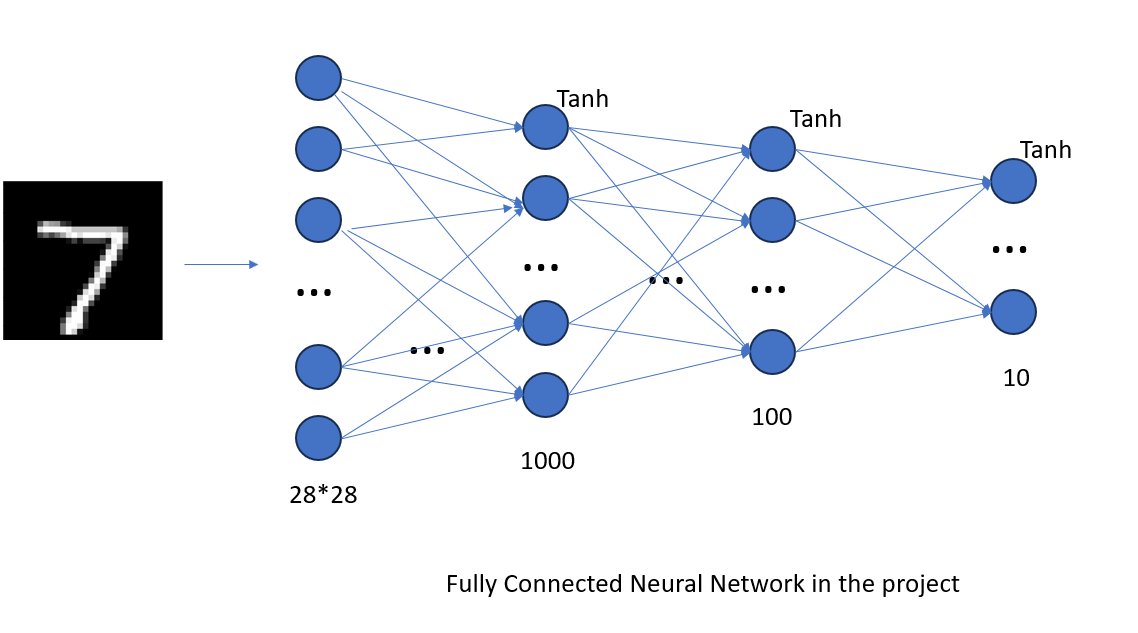
\includegraphics[width=0.6\textwidth]{FullyConnectedNN.PNG}
\end{center}
12. mnist-CNN: Test mnist data with Convolutional Neural Network. In this program, just 2 classes are used because we have convolutional computation in this program, so we need to reduce the number of classes for computation without GPU. Moreover, I want to use the binary cross-entropy loss functions for this project, so I chose 2 classes only for binary classification. The network for this file is illustrated below:
\begin{center}
    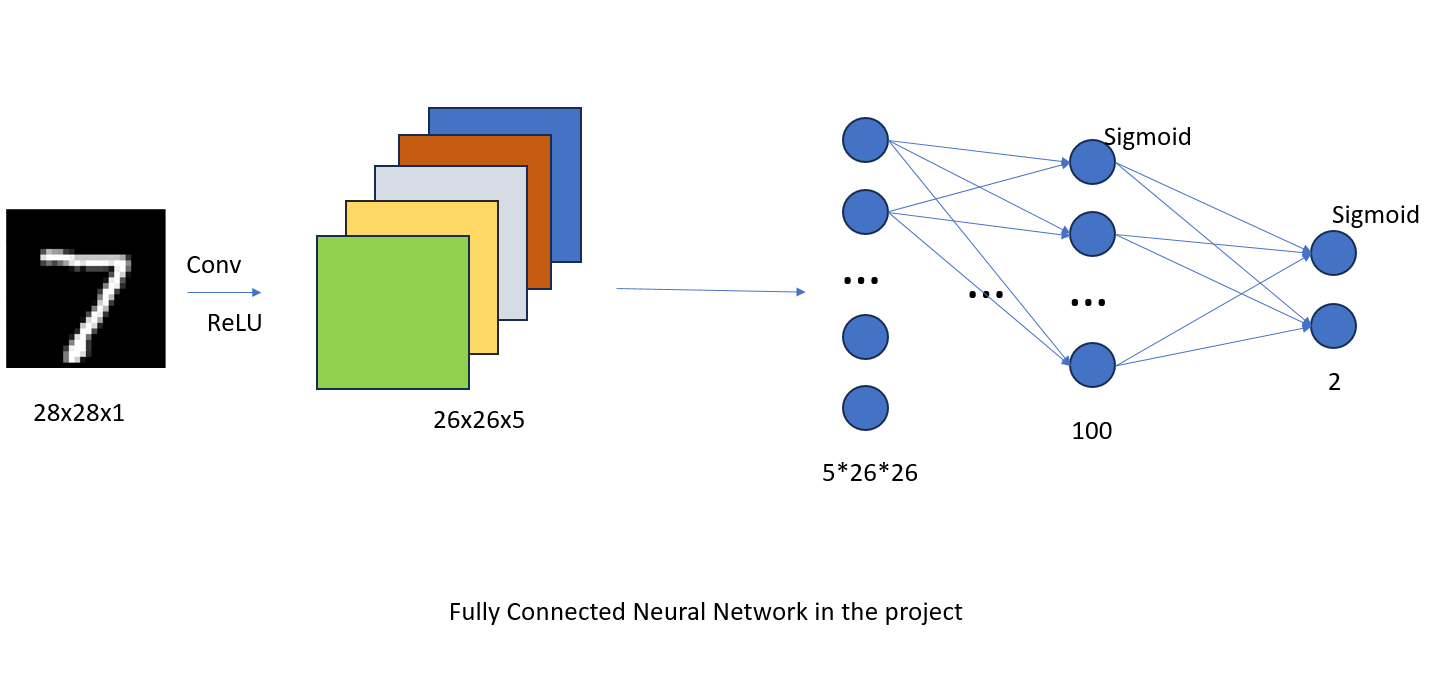
\includegraphics[width=0.6\textwidth]{SimpleCNN.PNG}
\end{center}
13. mnist-CNN-full: Test with layers that are available on code. The network for this file is illustrated below:
\begin{center}
    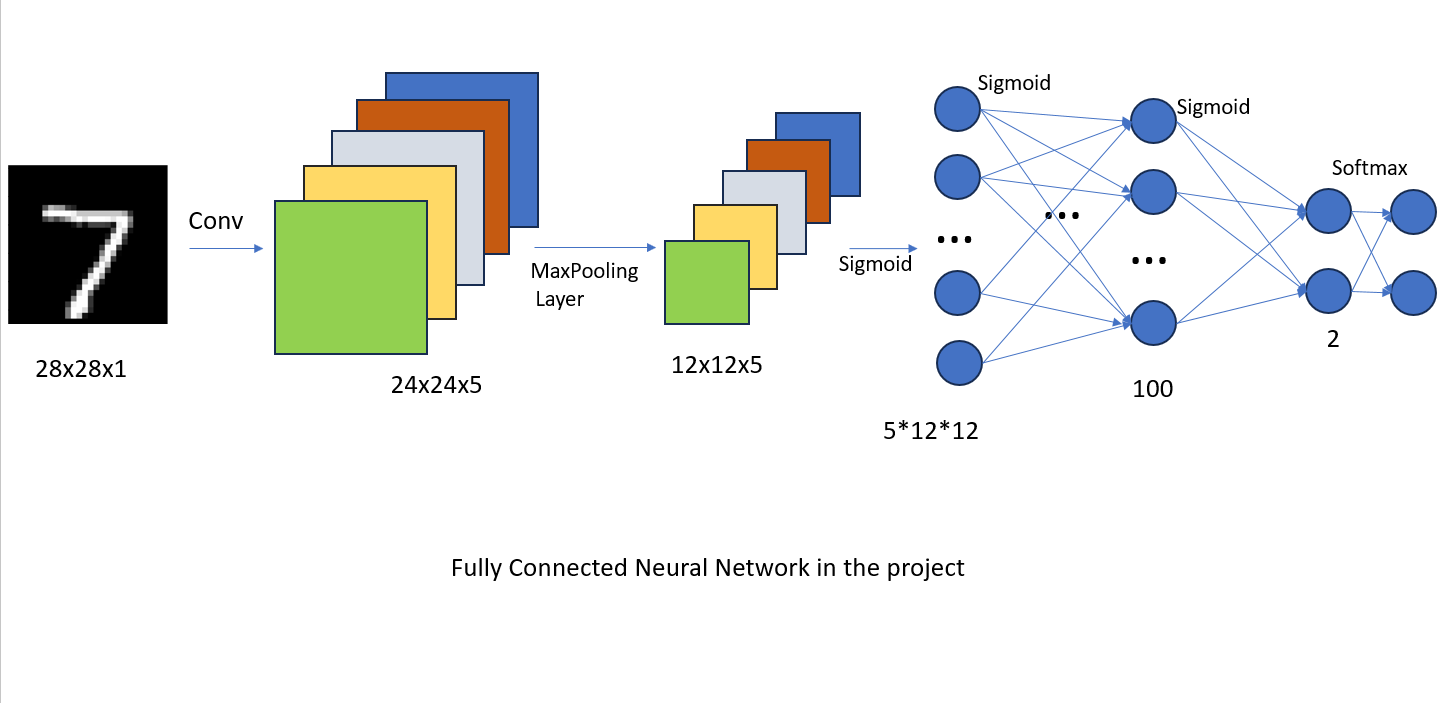
\includegraphics[width=0.6\textwidth]{CNN_full.PNG}
\end{center}
\section{Evaluation}
I created 2 CNNs with different layers and this is results of them when applying by mnist dataset:
\begin{figure}[!ht]
    \centering
    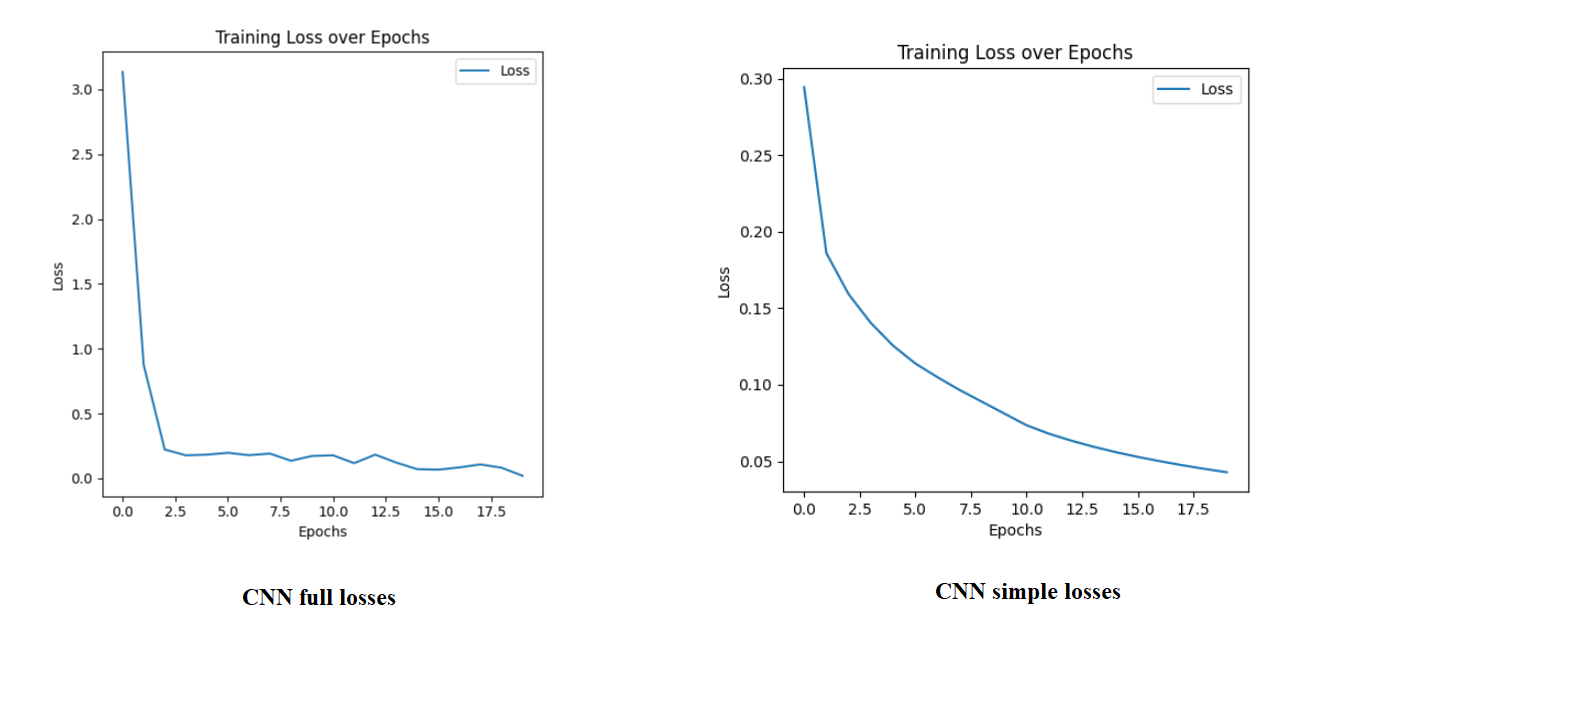
\includegraphics[width=\linewidth]{Comparison_between_losses.png}
    \caption{Comparison between losses}
    \label{fig:comparison_losses}
\end{figure}

\vspace{0.5cm} % Adjust the vertical space as needed
The value of loss of CNN simple smaller than CNN full at the beginning, but in the last epoch, the value of loss of CNN full is smaller. It caused because in the beginning, the CNN full is more complicated than CNN simple, so the error can be greater without training. However, after training process, we have smaller error by CNN full. \\
About the execution time, the execution time of CNN full smaller than CNN simple. Although CNN full have one more Layer "maxpooling", It reduces the size of the image from 24x24 to 12x12, reducing the link in the Dense.  In both CNNs, we can see they predicted well and the losses are acceptable. It means that the program worked correctly.\\

\clearpage % Forces a page break and flushes all pending floats

\begin{figure}[!ht]
    \centering
    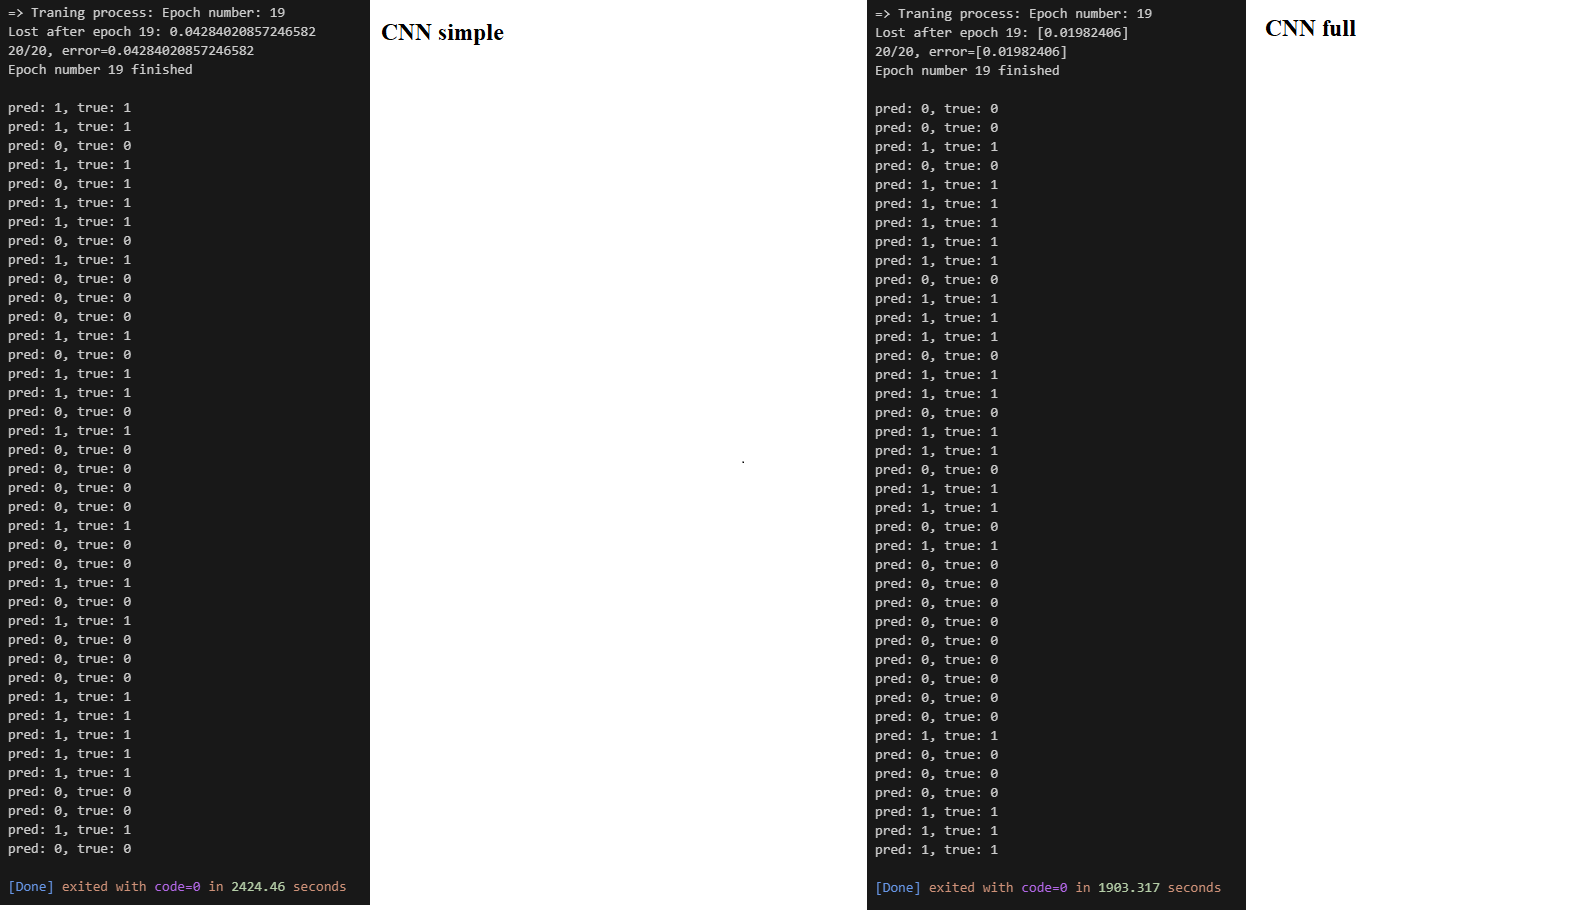
\includegraphics[width=\linewidth]{Comparison_between_final-loss_prediction_execution-time.png}
    \caption{Comparison between final loss, prediction and execution time}
    \label{fig:comparison_other_parameters}
\end{figure}

With Fully Connected NN, we have bad result by 2 reasons:\\
- The number of epochs is not enough. \\
- FCNN is not appropriate for image, because it does not have feature extraction and images are high dimentional data so if we apply FCNN for image, It require a massive number of parameters to connect every pixel to every neuron, which is computationally expensive and leads to overfitting. \\
Note: The result image of FCNN is in the end of the document. 
\begin{figure}[!ht]
    \centering
    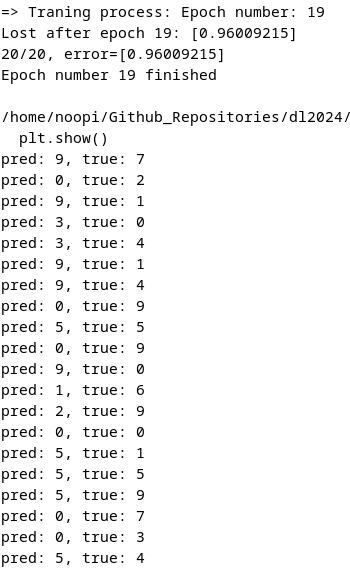
\includegraphics[width=\linewidth]{FCNN_last-epoch.png}
    \caption{Epoch number 20 of FCNN and its prediction}
    \label{fig:fcnn}
\end{figure}
\section{Conclusion}
\subsection{Challenges}
- Handle problems with tensors and matrices without numpy: It is really hard to handle matrices or tensors without numpy. In convolutional NN, we need to process matrices and tensors much, so it is necessary to create Helper from Linear Algebra to replace numpy from calculation in the project. However, matrices calculation from helper is inherited from other programs, so it is necessary to check format of the input (2D or 3D) in applying matrices calculation.  \\
- Linear Algebra problems: As I presented above, I programmed Helper for linear algebra task, but some time the error occur not because of algorithms, it occurs because of the format of the input, for example, some input has the format [[0.25] [1.5] [0.7] [3.0]] and it is in format of matrix but in Helper from LA, I programmed for elementwise multiply so it is a lot of conflict need to be fixed in the program. \\
- The other problems: Error of types, the differences of Softmax: we can not let Softmax inherit Activation because it has different format of input and returned value compared to other activation functions, etc.
\subsection{Observation after project}
- The knowledge about Deep Learning: important definitions, implementation from scratch, mathematical computation, convolutional calculation,... in Deep Learning. \\
- The importance of the recent libraries for solving problems with math, types,... \\
- The differences in calculation of convolutional network and fully connected network.\\
- Understand how CNN work, what happens in each layers, value of the nodes, how a CNN select features from data and optimize the parameters.
- The effect of layers to the model, then select appropriate input arguments for layers (for example, in Pooling Layer, I can not select to large kernel because the size of input image is small, if size of kernal is larger, it will lead to lost features of the input). 
\subsection{Results}
In this project, I implemented the Convolutional Neural Network without libraries and tested it with mnist dataset. The components of CNN have been programmed from scratch, and after testing, we can see that it worked well and the results appeared correctly.
\end{document}
